% ------------------------------------------------------------%
% 2015-2021 - Emerson Ribeiro de Mello <mello@ifsc.edu.br>
% ------------------------------------------------------------%
% Sets aspect ratio to 4:3, and frame size to 128 mm by 96 mm
\documentclass[aspectratio=169]{beamer}
% Sets aspect ratio to 16:9, and frame size to 160 mm by 90 mm.
% \documentclass[aspectratio=169]{beamer}
% Sets aspect ratio to 16:10, and frame size to 160 mm by 100 mm.
% \documentclass[aspectratio=1610]{beamer}
\usepackage[dvipsnames]{xcolor}
\usepackage{colortbl}
\usepackage{makecell}
\usepackage{multicol}
\usepackage{pifont}

\definecolor{DarkCyan}{HTML}{119DA4}
\definecolor{Asparagus}{HTML}{6DA34D}
\definecolor{CambridgeBlue}{HTML}{8FBC94}
\definecolor{TeaGreen}{HTML}{C5E99B}
\definecolor{Saphire}{HTML}{4059AD}



% -------------------------------------------------%
%  Package options
% -------------------------------------------------%
%  002625, EEE5E9, 0D1821, ADF7B6, B6C454
% textbgcolor   - frametitle background color. default: 0d4f4d
% textfgcolor   - frametitle foreground color. default: ffffff
% slidebgcolor  - slide background color. default: eef1ec
% slidefgcolor  - slide text foreground color. default: 000000
% authorfgcolor - author, institute and date color. default: 000000
% itemsep - space between items (itemize, enumerate). default: 7pt
\usepackage[textbgcolor=344966,textfgcolor=ffffff,slidebgcolor=EEE5E9,itemsep=7pt]{../0-ifscyan-modelo/beamerthemeifscyan}
% -------------------------------------------------%

% A good place to get some colors
% https://material.io/resources/color/#!/?view.left=0&view.right=0&primary.color=0d4f4d
% cyan: #0D4F4D, light: #417b79,  dark: #002625
% IFSC green: normal: #32A041, light: #69d26f, dark: #007013
% IFSC red: normal: #C8191E, light: #ff5747, dark: #8f0000 
% Other colors for textbgcolor
% purple 4527a0, blue 0d47a1, grey 546e7a, redwine 880e4f, brown 6d4c41, yelllow (bg=#fbc02d, fg=000000)

% Logo
\pgfdeclareimage[height=.3\paperheight]{ifpilogo}{../0-ifscyan-modelo/figs/Logo-IFPI-Vertical.png}

\AtBeginSection[]{
  \begin{frame}
  \vfill
  \centering
  \begin{beamercolorbox}[sep=8pt,center,shadow=true,rounded=true]{title}
    \usebeamerfont{title}\insertsectionhead\par%
  \end{beamercolorbox}
  \vfill
  \end{frame}
}

% -------------------------------------------------%
%              Título 
% -------------------------------------------------%
\title{Matemática Computacional}
\subtitle{Análise Combinatória - Arranjos e Combinações Simples}
\author{Prof. Rogério Figueredo de Sousa}
\institute{%
\href{rogerio.sousa@ifpi.edu.br}{rogerio.sousa@ifpi.edu.br}%
}%
\date{10/09/2024}
% -------------------------------------------------%

% -------------------------------------------------%
%  Início do documento 
% -------------------------------------------------%
\begin{document}

\begin{frame}[plain]
    \titlepage
\end{frame}

%\begin{frame}[plain, noframenumbering]{Licenciamento}
%    \licenciamentoLivre
%\end{frame}

%\begin{frame}[plain, noframenumbering]{Sumário}
%   \tableofcontents
%\end{frame}


\jsonp
\lstset{
    numbers=none,
    escapeinside={\%*}{*)},
}
\section{Arranjo Simples}
%1
\begin{frame}{Arranjo Simples: Introdução}

\textbf{    Exemplo 1:}

    \vspace{4mm}
    \begin{itemize}
        \item[] Um prédio tem 8 portas. De quantas maneiras 1 pessoa pode entrar por 1 porta e sair por outra diferente?
    \end{itemize}

    \pause
    \vspace{4mm}

   \textbf{ Resolução:}

    \begin{center}
        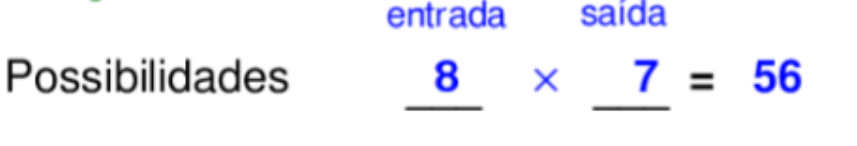
\includegraphics[width=0.5\linewidth]{figs/Exemplo01.png}
    \end{center}

    \textbf{Resposta:}

    \begin{itemize}
        \item[] Uma pessoa pode entrar por uma porta e sair por outra de \textbf{56 maneiras distintas}.
    \end{itemize}

\end{frame}

%2
\begin{frame}{Arranjo Simples: Introdução}

    \textbf{Reformulação do Exemplo 1:}
    
        \vspace{4mm}
        \begin{itemize}
            \item Um prédio tem 8 portas. De quantas maneiras 1 pessoa pode entrar por 1 porta e sair por outra diferente?
            \item De \underline{quantas maneiras distintas} uma pessoa pode escolher \underline{2} portas \underline{diferentes} (entrada, saída) entre \underline{8} portas \underline{diferentes}?
        \end{itemize}
    
        \vspace{2mm}
    
       \textbf{ Resposta:}
    
        \begin{itemize}
            \item[] Uma pessoa pode entrar por uma porta e sair por outra de \textbf{56 maneiras distintas}.
        \end{itemize}

        \vspace{2mm}
        \textbf{ Resposta:}

        \begin{itemize}
            \item[] Uma pessoa pode escolher \underline{2} portas \underline{distintas} para entrar e sair entre \underline{8} portas \underline{distintas} de 56 maneiras diferentes.
        \end{itemize}

        \vspace{2mm}

        Observação: $8 \cdot 7$ \pause $ = \frac{8 \cdot 7 \cdot 6!}{6!}$ \pause $= \frac{8 \cdot 7 \cdot 6 \cdot 5 \cdot 4 \cdot 3 \cdot 2 \cdot 1}{6!}$ \pause $ = \frac{8!}{6!}$ \pause $ = \frac{8!}{(8 - 2)!}$
    

    \end{frame}

%3
\begin{frame}{Arranjo Simples}

    \textbf{Exemplo 2:}
    
        \vspace{4mm}
        \begin{itemize}
            \item[] Quantos números distinos de 3 algarismos distintos podem se formar com os dígitos 3, 5, 7, 8 e 9?
        \end{itemize}
    
        \vspace{2mm}
    
       \textbf{Resolução:}
        
       \begin{multicols}{2}
           
        \begin{center}
            Possibilidades
        \end{center}
            
            
        \columnbreak

        
        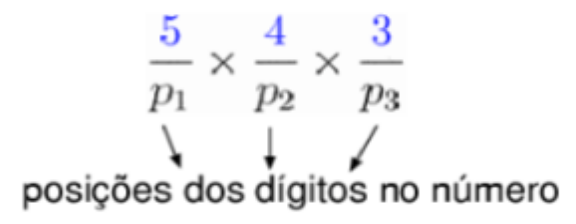
\includegraphics[width=0.6\linewidth]{figs/Exemplo02.png}
            
           
       \end{multicols}
        
    
        \textbf{Resposta:}
    
        \begin{itemize}
            \item[] Podem se formar $5 \cdot 4 \cdot 3 = 60$ números diferentes com 3 algarismos escolhidos entre os dígitos 3, 5, 7, 8 e 9.
        \end{itemize}
    
        \vspace{2mm}

        Observação: $5 \cdot 4 \cdot 3 = \frac{5 \cdot 4 \cdot 3 \cdot 2}{2!} = \frac{5!}{2!} = \frac{5!}{(5 - 3)!}$
    \end{frame}

%4
\begin{frame}{Arranjo Simples}
    \begin{itemize}
        \item Características dos exemplos:
        \begin{itemize}
            \item Os elementos considerados $a_1, a_2, \ldots, a_n$ são diferentes.
            \item Cada escolha de r elementos ($r \leq n$) distintos e ordenados entre $a_1, a_2, \ldots, a_n$ corresponde a uma possibilidade.
            \item Na obtenção do número de possibilidades aplica-se os princípios aditivo e multiplicativo.
        \end{itemize}
    \end{itemize}
\end{frame}

%4
\begin{frame}{Arranjo Simples}
    \begin{itemize}
        \item Definição:
        \begin{itemize}
            \item Dados n objetos distintos $a_1, a_2, \ldots, a_n$, um arranjo simples de n elementos tomados \textbf{r} a \textbf{r} é uma ordenação de \textbf{r} elementos distintos escolhidos entre $a_1, a_2, \ldots, a_n$, sendo \textbf{r} e \textbf{n} números naturais com $1 \leq r \leq n$.
        \end{itemize}
    \end{itemize}

    \vspace{4mm}
    \begin{itemize}
        \item Ilustração:
        \begin{itemize}
            \item Dados os dígitos 3,5,7,8 e 9, \textbf{398 é um arranjo simples} de \underline{5} elementos tomados \underline{3 a 3}.
        \end{itemize}
    \end{itemize}


\end{frame}

%5
\begin{frame}{Arranjo Simples}
    \begin{itemize}
        \item Problema:
        \begin{itemize}
            \item \underline{Dados} n objetos distintos $a_1, a_2, \ldots, a_n$,
            \item \underline{encontrar} o número de arranjos simples dos n elementos tomados de \textbf{r} a \textbf{r}.
        \end{itemize}
    \end{itemize}

    \vspace{4mm}
    \begin{itemize}
        \item Propriedade:
        \begin{itemize}
            \item O número de \underline{arranjos simples} de n elementos distintos tomados \textbf{r} a \textbf{r}, denominado $A(n, r)$, é dado por:
        \end{itemize}
    \end{itemize}

    $$ A(n,r) = n(n-1)\ldots(n-(r-1)) = \frac{n!}{(n-r)!}$$

    \vspace{4mm}
    \begin{itemize}
        \item Observação:
    \end{itemize}

    $$ P_n = A(n,n) = n! $$

\end{frame}

%7
\begin{frame}{Arranjo Simples}
    \textbf{Exemplo 3:}
    \vspace{4mm}

    \begin{itemize}
        \item[] Vários amigos combinaram passar o dia no clube. Planejaram ir para a piscina, fazer um churrasco, jogar volei e tennis. Mas, como chegaram tarde precisaram escolher 3 entre as 4 atividades. De quantas maneiras diferentes poderiam reprogramar essas atividades?
    \end{itemize}

    \vspace{2mm}
    \pause
    \textbf{Resolução:}
    \begin{itemize}
        \item[] \textbf{Programa:} arranjo simples de 3 atividades escolhidas entre 4 \pause
        \item[] \textbf{Número de programas possíveis:} $ A (4,3) = \frac{4!}{(4-3)!} = 4! = 24$
    \end{itemize}

    \pause
    \vspace{2mm}
    \textbf{Resposta:}

    \begin{itemize}
        \item[] Eles têm 24 maneiras diferentes de fazer um programa.
    \end{itemize}
\end{frame}

%8
\begin{frame}{Arranjo Simples}
    \textbf{Exemplo 4:}
    \vspace{2mm}

    \begin{itemize}
        \item[] Uma companhia aérea tem vôos ligando 5 cidades. Cada rota interliga 3 cidades. Calcule o número de rotas diferentes.
    \end{itemize}

    \vspace{2mm}
    \pause
    \textbf{Ilustração:}
    
    \begin{center}
        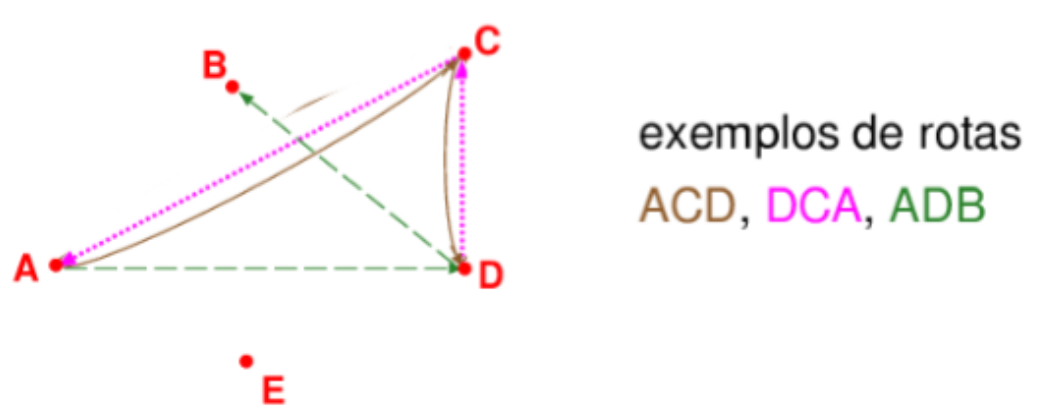
\includegraphics[width=.8\linewidth]{figs/Exemplo04.png}
    \end{center}
\end{frame}

%9
\begin{frame}{Arranjo Simples}
    \textbf{Resolução:}
    \vspace{2mm}

    \begin{center}
        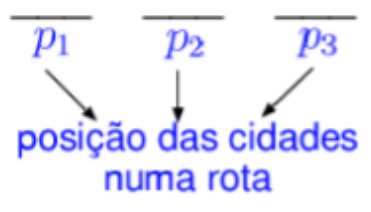
\includegraphics[width=.3\linewidth]{figs/Exemplo04_1.png}
    \end{center}

    \pause
    \begin{itemize}
        \item Rota: Arranjo simples de 3 cidades escolhidas entre 5. \pause
        \item Número de rotas: $A(5,3) = \frac{5!}{(5-3)!} = \frac{5!}{2!} = 5 \cdot 4 \cdot 3 = 60$ 
    \end{itemize}

    \vspace{2mm}
    \pause
    \textbf{Resposta:}
    
    \begin{itemize}
        \item[] A companhia pode ter 60 rotas ligando as 5 cidades.
    \end{itemize}
\end{frame}


%8
\begin{frame}{Arranjo Simples}
    \textbf{Exemplo 5:}
    \vspace{2mm}

    \begin{itemize}
        \item[] As placas dos automóveis são formadas por três letras seguidas de quatro dígitos. Quantas placas com letras e números diferentes podem ser formadas?
    \end{itemize}

    \vspace{2mm}
    \pause
    \textbf{Resolução:}
    
    \begin{multicols}{2}
        \begin{center}
            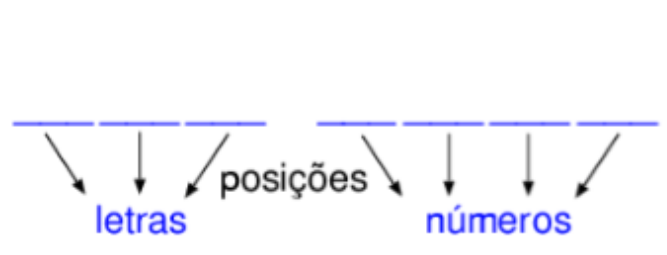
\includegraphics[width=.9\linewidth]{figs/Exemplo05.png}
        \end{center}
        
        \pause
        \columnbreak

        \begin{itemize}
            \item[] número de letras = 26 \pause
            \item[] número de letras numa placa = 3 \pause
            \item[] número de dígitos = 10 \pause
            \item[] número de dígitos numa placa = 4
        \end{itemize}
    \end{multicols}

    
\end{frame}

%11
\begin{frame}{Arranjo Simples}
    \textbf{Característica:}
    \vspace{2mm}

    \begin{multicols}{2}
        \begin{center}
            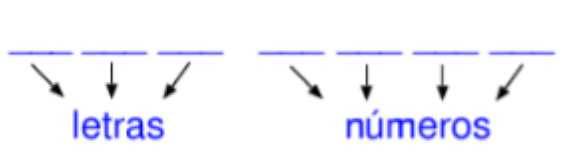
\includegraphics[width=.8\linewidth]{figs/Exemplo05_1.png}
        \end{center}
        
        \pause
        \columnbreak

        \begin{itemize}
            \item Pares ordenados de 3 letras e 4 números
        \end{itemize}
    \end{multicols}

    \vspace{2mm}
    \pause
    \textbf{Número de possibilidades:}
    
    
        \begin{itemize}
            \item[] \hspace{1mm} letras \hspace{10mm} números \pause
            \item[] $A(26,3)$ \hspace{2.5mm} \pause $\times$ \hspace{2mm} $A(10,4)$  \pause $= \frac{26!}{23!} \times \frac{10!}{6!} = 78624 \times 10^3$
        \end{itemize}

    \pause
    \textbf{Resposta:}

    \vspace{2mm}

    \begin{itemize}
        \item Tem-se 78624000 placas com 3 letras e 4 números diferentes
    \end{itemize}

    
\end{frame}

%12
\begin{frame}{Arranjo Simples}
    \textbf{Exemplo 6:}
    \vspace{2mm}

    \begin{itemize}
        \item[] Quantos números naturais de três algarismos distintos (na base 10) existem?
    \end{itemize}

    \vspace{2mm}
    \pause
    \textbf{Resolução:}
    
    \begin{itemize}
        \item dígitos? 0, 1, 2, 3, 4, 5, 6, 7, 8, 9 \pause
    \end{itemize}

    \begin{center}
        
\includegraphics[width=0.2\linewidth]{figs/Exemplo06.png}
    \end{center}

    \vspace{4mm}

    \begin{itemize}
        \item[] Raciocínio 1: \hspace{2.2cm} 
\includegraphics[width=0.25\linewidth]{figs/Exemplo06_1.png}
        \item[] Possibilidades: \hspace{2.2cm} $9$ \hspace{0.2cm} $\times$ \hspace{0.4cm} $A(9,2)$ $ = 9 \cdot 9 \cdot 8 = 648$ 
    \end{itemize}
    
\end{frame}


%13
\begin{frame}{Arranjo Simples}
    \textbf{Exemplo 6 (raciocínio 2):}
    \vspace{2mm}

    \begin{itemize}
        \item[] Usamos o conceito de complemento:
        \item U := conjunto universo := o conjunto das ordenações de três dígitos
        \item A := conjunto dos números de 3 algarismos.
        \item B := conjunto dos elementos de U que iniciam com 0 
        \begin{itemize}
            \item $A = U - B$
            \item $N = |A| = |U| - |B|$
        \end{itemize}
        \vspace{2mm}
        \pause 
        \begin{itemize}
            \item $|U| = A(10,3) = \frac{10!}{7!}, |B| = A(9,2) = \frac{9!}{7!}$
            \item $N = \frac{10!}{7!} - \frac{9!}{7!} = \frac{10 \cdot 9! - 9!}{7!} = 648$
        \end{itemize}
    \end{itemize}

    \vspace{2mm}
    \pause
    \textbf{Resposta:}
    
    \begin{itemize}
        \item Tem-se 648 números naturais de três algarismos distintos.
    \end{itemize}

    
\end{frame}


%14
\begin{frame}{Arranjo Simples}
    

    \begin{itemize}
        \item Recomendação
        \vspace{4mm}
        \begin{itemize}
            \item Em geral é conveniente começar a análise dos eventos (ou possibilidades) por aquelas que tem algum tipo de impedimento (ou dificuldade)
        \end{itemize}
    \end{itemize}

\end{frame}

%15
\begin{frame}{Arranjo Simples}
    \textbf{Exemplo 7:}

    \begin{itemize}
        \item[] Quantos números naturais com todos os dígitos distintos ímpares, m, existem entre 1000 e 9999 (1000 < m < 9999)?
    \end{itemize}

    \vspace{2mm}
    \pause
    \textbf{Resolução:}
    
    \begin{multicols}{2}
        \begin{itemize}
            \item Os números m tem 4 dígitos \pause
            \item Dígitos ímpares: 1,3,5,7,9             
        \end{itemize}

        \columnbreak

        \begin{center}
            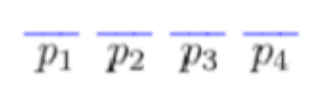
\includegraphics[width=0.4\linewidth]{figs/Exemplo07.png}
        \end{center}
    \end{multicols}

    \begin{itemize}
        \item[] n: quantidade de dígitos ímpares = 5 \pause
        \item[] r: quantidade de dígitos de um número = 4
        
    \end{itemize}

    \pause 
    \vspace{2mm}
    \textbf{Possibilidades:} $A(5,4) = \frac{5!}{(5-4)!} = 5! = 5 \cdot 4 \cdot 3 \cdot 2 \cdot 1 = 120$

    \textbf{Resposta:} Existem 120 números com todos os dígitos distintos ímpares entre 1000 e 9999.
\end{frame}


%16
\begin{frame}{Arranjo Simples}
    

    \begin{itemize}
        \item Observação
        \vspace{4mm}
        $$A(5,4) = \frac{5!}{(5-4)!} = 5! = P_5 = A(5,5) = \frac{5!}{(5 - 5)!}$$

        \begin{itemize}
            \item \underline{Em geral},
            \vspace{4mm}
                
            
        \end{itemize}
        $$A(n,n-1) = A(n,n) = P_n = n!$$
    \end{itemize}

\end{frame}


%17
\begin{frame}{Arranjo Simples}
    \textbf{Exemplo 8:}

    \begin{itemize}
        \item[] Quantos números pares de quatro dígitos têm dígitos distintos?
    \end{itemize}

    \vspace{2mm}
    \pause
    \textbf{Resolução:}
    
   \begin{center}
            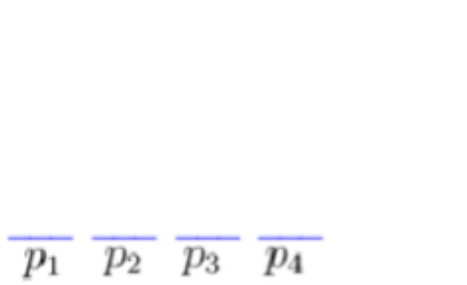
\includegraphics[width=0.3\linewidth]{figs/Exemplo08.png}
    \end{center}

\end{frame}

%17
\begin{frame}{Arranjo Simples}
    \textbf{Exemplo 8:}

    \begin{itemize}
        \item[] Quantos números pares de quatro dígitos têm dígitos distintos?
    \end{itemize}

    \vspace{2mm}
    
    \textbf{Resolução:}
    
   \begin{center}
            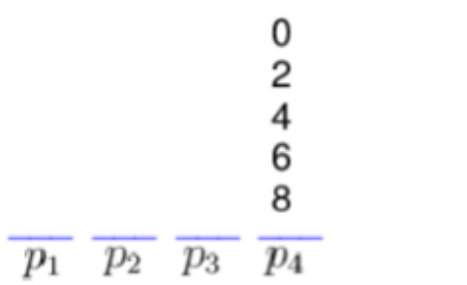
\includegraphics[width=0.3\linewidth]{figs/Exemplo08_1.png}
    \end{center}

\end{frame}

%17
\begin{frame}{Arranjo Simples}
    \textbf{Exemplo 8:}

    \begin{itemize}
        \item[] Quantos números pares de quatro dígitos têm dígitos distintos?
    \end{itemize}

    \vspace{2mm}
    
    \textbf{Resolução:}
    
   \begin{center}
            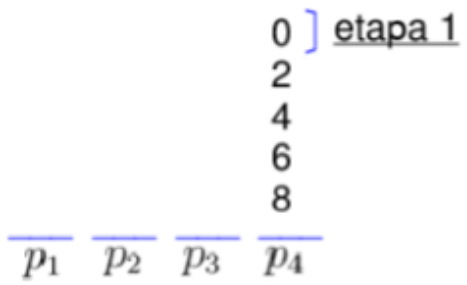
\includegraphics[width=0.3\linewidth]{figs/Exemplo08_2.png}
    \end{center}
\end{frame}


%20
\begin{frame}{Arranjo Simples}
    \textbf{Exemplo 8:}

    \begin{itemize}
        \item[] Quantos números pares de quatro dígitos têm dígitos distintos?
    \end{itemize}

    \vspace{2mm}
    
    \textbf{Resolução:}
    
   \begin{center}
            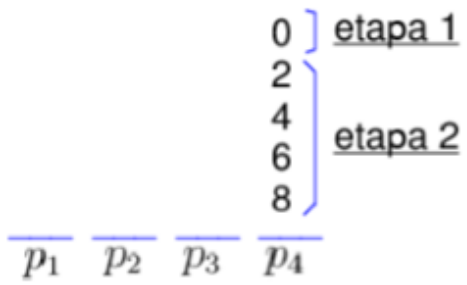
\includegraphics[width=0.3\linewidth]{figs/Exemplo08_3.png}
    \end{center}

    \pause
    \begin{itemize}
        \item[] M: quantidade de números naturais de 4 dígitos terminados em 0, 2, 4, 6 ou 8. \pause
        \item[] $M = M_1 + M_2$, sendo
        \item[] $M_1$: quantidade de números de 4 dígitos terminados em 0 (etapa 1)
        \item[] $M_2$: quantidade de números de 4 dígitos terminados em 2, 4, 6 ou 8 (etapa 2)
    \end{itemize}

\end{frame}

%22
\begin{frame}{Arranjo Simples}
    \textbf{Exemplo 8 (etapa 1):}

    \begin{itemize}
        \item[] Obtenção de $M_1$, quantidade de números de dígitos distintos, com 4 dígitos terminados em 0:
    \end{itemize}

    \vspace{2mm}
    
    \pause
    \textbf{Possibilidades:} \hspace{1cm} 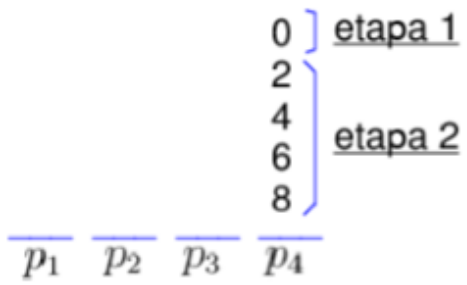
\includegraphics[width=0.3\linewidth]{figs/Exemplo08_3.png}
    
   \pause
    \begin{itemize}
        \item[] Como $A(n,r) = n(n-1) \ldots (n-(r-1))$
        \item[] \hspace{1cm} $n = 9$, $r = 3$
    \end{itemize}

\end{frame}

%23
\begin{frame}{Arranjo Simples}
    \textbf{Exemplo 8 (etapa 2):}

    \begin{itemize}
        \item[] Obtenção de $M_2$, quantidade de números de dígitos distintos, entre 1000 e 9999 terminados em 2, 4, 6 ou 8:
    \end{itemize}

    \vspace{2mm}
    
    \pause
    \textbf{Possibilidades:} \hspace{2cm} 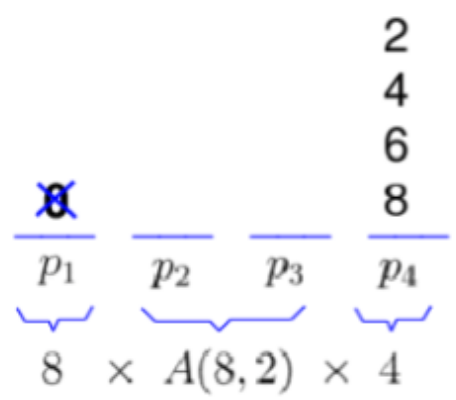
\includegraphics[width=0.3\linewidth]{figs/Exemplo08_4.png}
    
   \pause

   \vspace{4mm}

   \textbf{Resposta da etapa 2:} $M_2 = 8 \cdot 8 \cdot 7 \cdot 4$

\end{frame}

%24
\begin{frame}{Arranjo Simples}
    \textbf{Exemplo 8 (análise final):}

    \begin{itemize}
        \item[] Enunciado: Quantos números naturais entre 1000 e 9999 têm dígitos distintos e são pares?
        \item[] Resolução:
        \begin{itemize}
            \item $M = M_1 + M_2$, sendo
            \item M: total de números naturais de 4 dígitos terminados em 0, 2, 4, 6 ou 8
            \item $M_1$: total de números de 4 dígitos terminados em 0 (etapa 1)
            \item $M_2$: total de números de 4 dígitos terminados em 2, 4, 6 ou 8 (etapa 2)
        \end{itemize}
    \end{itemize}

    \pause
    \textbf{Resposta:} 
    
    \begin{itemize}
        \item Como, $M_1 = A(9,3) = 504, M_2 = 8 \cdot 4 \cdot A(8,2) = 1792$ tem-se que $M = 504 + 1792 = 2296$
    \end{itemize}
    

\end{frame}

\section{Combinações Simples}

%24
\begin{frame}{Combinações Simples: Introdução}
    \textbf{Exemplo 1:} 
    \begin{itemize}
        \item[] Numa sala estão reunidas três pessoas, $P_1, P_2$ e $P_3$. De quantas maneiras podemos selecionar \underline{duas} pessoas?
    \end{itemize}

    \pause
    \textbf{Reformulação do exemplo:} 
    
    \begin{itemize}
        \item[] Seja $A = \{P_1, P_2, P_3\}$. Quantos subconjuntos de 2 elementos possui A?
    \end{itemize}
    

\end{frame}

%24
\begin{frame}{Combinações Simples: Introdução}
    \textbf{Exemplo 1 (continuação):} 

    \begin{itemize}
        \item[] \textbf{Resolução:}
        \begin{itemize}
            \item[] $$A = \{P_1, P_2, P_3\}$$ \vspace{2mm} \pause
            \item N: número de subconjuntos de 2 elementos de A
            \item \underline{Raciocínio 1}: enumeração dos subconjuntos de A
            \item[] $$B = \{\{P_1, P_2\}, \{P_1, P_3\}, \{P_2, P_3\}\}$$ \pause
            \item \textbf{Resposta:}
        \end{itemize}
    \end{itemize}

    $$ N = |B| = n(B) = 3$$
\end{frame}

%29
\begin{frame}{Combinações Simples: Introdução}
    \textbf{Exemplo 1 (raciocínio 2):} 

    \begin{itemize}
        \item[] Sem enumeração dos subconjuntos de A (usando arranjos e permutações)
        \vspace{2mm}
        \item Os arranjos de 3 elementos tomados 2 a 2 consideram a ordem!
        \vspace{2mm}
        \item Então \underline{devemos} reduzir a 1 possibilidade todas as permutações dos mesmos elementos.
    \end{itemize}

\end{frame}

%30
\begin{frame}{Combinações Simples: Introdução}
    \textbf{Exemplo 1 (continuação):} 

    \begin{itemize} 
        \item[] $A(3,2)$
    \end{itemize}

    \begin{center}
        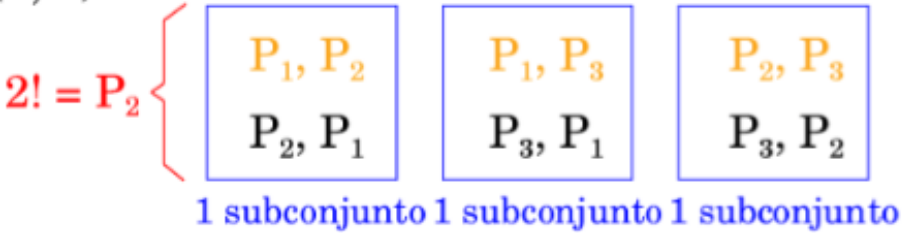
\includegraphics[width=0.5\linewidth]{figs/Comb_exemplo01.png}
    \end{center}

    \pause
    \vspace{2mm}

    \textbf{Resumindo:}

    \begin{itemize}
        \item[] $P_2$ \hspace{1cm} 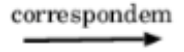
\includegraphics[width=0.1\linewidth]{figs/Comb_exemplo01_1.png} \hspace{1cm} 1 subconjunto \pause
        \item[] $A(3,2)$ \hspace{0.3cm} 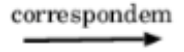
\includegraphics[width=0.1\linewidth]{figs/Comb_exemplo01_1.png} \hspace{1cm} $N = \frac{A(3,2)}{P_2}$ total de subconjuntos \pause
    \end{itemize}

    \vspace{2mm}

    \textbf{Resposta:}

    $$ N = \frac{A(3,2)}{P_2} = \frac{3!}{2! (3-2)!} = \frac{3 \cdot 2!}{2! \cdot 1!} = 3$$


\end{frame}

%31
\begin{frame}{Combinações Simples}
    \textbf{Exemplo 2:} 

    \begin{itemize}
        \item[] Uma fábrica de sucos está lançando no mercado 5 novos sabores. Como propaganda, cada pessoa pode experimentar 2 sabores diferentes. Quantas opções tem cada um?
    \end{itemize}

    \pause
    \textbf{Resolução:}

    \begin{center}
        
    $S_1, S_2, S_3, S_4, S_5$
\end{center}

\pause
    \begin{itemize}
        \item 1 opção: uma escolha de 2 sabores entre 5 (não importa a ordem)
        \item N: número de opções \pause
    \end{itemize}

    \begin{itemize}
        \item[] $P_2$ \hspace{1cm} 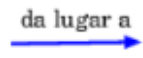
\includegraphics[width=0.1\linewidth]{figs/Comb_exemplo02.png} \hspace{1cm} 1 opção \pause
        \item[] $A(5,2)$ \hspace{0.3cm} 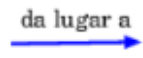
\includegraphics[width=0.1\linewidth]{figs/Comb_exemplo02.png} \hspace{1cm} N opções = $\frac{A(5,2)}{P_2}$ 
    \end{itemize}

    \pause
     \textbf{Resposta:}

    $$ N = \frac{A(5,2)}{P_2} = \frac{5!}{2! (5-2)!} = \frac{5}{2! \cdot 3!} = 10$$


\end{frame}


%32
\begin{frame}{Combinações Simples}
    \begin{itemize}
        \item[] Características dos exemplos
        \begin{itemize}
            \item Os elementos considerados $a_1, a_2, \ldots, a_n$ são diferentes.
            \item Cada escolha de r elementos distintos (sem importar a ordem) entre $a_1, a_2 , \ldots, a_n$ corresponde a uma possibilidade.
            \item Na obtenção do número de possibilidades aplica-se os princípios aditivo e multiplicativo (usa-se os conceitos de arranjos e permutações).
        \end{itemize}
    \end{itemize}

\end{frame}



%33
\begin{frame}{Combinações Simples}
    \begin{itemize}
        \item Definição:
        \begin{itemize}
            \item Dados n objetos distintos $a_1, a_2, \ldots, a_n$, uma combinação simples de n elementos tomados de r a r é uma seleção de r elementos distintos escolhidos entre $a_1, a_2, \ldots, a_n$, não importando a ordem da escolha, sendo r e n números naturais com $1 \leq r \leq n$.
        \end{itemize}
        \item Ilustração:
        \begin{itemize}
            \item Dadas as pessoas $P_1, P_2, P_3$, 
            \item $P_1, P_3$ é uma combinação de 3 elementos tomados de 2 a 2.
        \end{itemize}
    \end{itemize}
\end{frame}


%33
\begin{frame}{Número de Combinações Simples}
    \begin{itemize}
        \item Problema:
        \begin{itemize}
            \item[] \underline{Dados} n elementos ditintos, $a_1, a_2, \ldots, a_n$,
            \item[] \underline{encontrar} o número de combinações simples dos n elementos tomados r a r.
        \end{itemize}
        \item Propriedade:
        \begin{itemize}
            \item O número de combinações simples de n elementos distintos tomados de r a r, denominado C(n,r), é:
            
            $$ C(n,r) = \frac{n!}{r! (n-r)!} = \frac{A(n,r)}{P_r}$$
        \end{itemize}
        \item Observação:
        
            $$ C(n,r) = C(n, n - r ) = \frac{n!}{(n-r)! (n - (n-r))!}$$
        
    \end{itemize}
\end{frame}

%35
\begin{frame}{Número de Combinações Simples}
    \textbf{Exemplo 3:}
    \begin{itemize}
        \item[] Um técnico convocou 9 jogadores para um campeonato de vôlei. Para formar a equipe inicial deve escolher 5 jogadores. Quantas opções ele tem?
    \end{itemize}

    \pause
    \vspace{2mm}

    \textbf{Resolução:}

    \begin{itemize}
        \item[] n = número de jogadores = 9 \pause
        \item[] r = número de jogadores da equipe = 5 \pause
        \item[] total de opções:
    \end{itemize}

    $$ C(9,5) = \frac{9!}{5! (9-5)!} = \frac{9 \cdot8 \cdot 7 \cdot 6 \cdot 5!}{5! \cdot 4 \cdot 3 \cdot 2} = 9 \cdot 2 \cdot 7 = 126$$

    \textbf{Resposta:}
    \begin{itemize}
        \item[] O técnico tem 126 opções de formar a equipe inicial.
    \end{itemize}
\end{frame}

%36
\begin{frame}{Número de Combinações Simples}
    \textbf{Exemplo 4:}
    \begin{itemize}
        \item[] Um grupo de trabalho tem 12 professores do curso de informática e 12 professores do curso de matemática. Quantas comissões de 8 professores podem ser formadas?
    \end{itemize}

    \pause
    \vspace{2mm}

    \textbf{Resolução:}

    \begin{itemize}
        \item[] n = número de professores = $12 + 12 = 24$ \pause
        \item[] r = número de professores em uma comissão = 8 \pause
        \item[] N: Numero de comissões possíveis
    \end{itemize}

    \pause
    \textbf{Resposta:}
    \begin{itemize}
        \item[] Podem ser formadas:
    \end{itemize}

    $$ N = C(24,8) = \frac{24!}{8! 16!} = \frac{24 \cdot 23 \cdot 22 \cdot 21 \cdot 20 \cdot 19 \cdot 18 \cdot 17}{8 \cdot 7 \cdot 6 \cdot 5 \cdot 4 \cdot 3 \cdot 2} = 735471 ~ comiss\tilde{o}es$$  .

\end{frame}

%37
\begin{frame}{Número de Combinações Simples}
    \textbf{Exemplo 5:}
    \begin{itemize}
        \item[] Um grupo de trabalho tem 12 professores do curso de informática e 12 professores do curso de matemática. Quantas comissões de 8 professores podem ser formadas havendo 3 professores de matemática?
    \end{itemize}

    \pause
    \vspace{2mm}

    \textbf{Resolução:}

    \begin{itemize}
        \item[] número de professores = $12 + 12 = 24$ \pause
        \item[] número de professores de matemática em uma comissão = 3 \pause
        \item[] número de professores de informática em uma comissão = 8 - 3 = 5
    \end{itemize}

    \pause
    \textbf{Possibilidades:} $\frac{C(12,3)}{matem\acute{a}tica ~ (3 ~ de ~ 12)} \times \frac{C(12,5)}{inform\acute{a}tica ~ (5 ~ de ~ 12)} = \frac{12!}{3! 9!} \times \frac{12!}{5! 7!}$

    \vspace{2mm}
    \textbf{Resposta:}
    \begin{itemize}
        \item[] O número de comissões é 174240.
    \end{itemize}
\end{frame}


%38
\begin{frame}{Número de Combinações Simples}
    \textbf{Exemplo 6:}
    \begin{itemize}
        \item[] Um grupo de trabalho tem 12 professores do curso de informática e 12 professores do curso de matemática. Quantas comissões de 8 professores podem ser formadas havendo pelo menos 1 professor de matemática?
    \end{itemize}

    \pause
    \vspace{2mm}

    \textbf{Resolução:}

    \begin{itemize}
        \item Raciocínio 1:
        \begin{itemize}
        \item[] U: conjunto universo := o conjunto de todas as comissões de 8 professores  \pause
        \item[] A:= conjunto de todas as comissões com pelo menos 1 professor de matemática \pause
        \item[] B:= conjunto de todas as comissões sem professor de matemática
        \end{itemize}
    \end{itemize}

\end{frame}


%39
\begin{frame}{Número de Combinações Simples}
    \textbf{Exemplo 6 (continuação):}
    \begin{itemize}
        \item[] $A = U - B$
        \item[] número de comissões := $N = |A| = |U| = |B|$
    \end{itemize}

    \pause
    \vspace{2mm}

    \begin{itemize}
        \item[] $|U|$  \pause $= C(24,8)$, \pause $|B|$ \pause $= C(12,8)$ \pause
        \item[] $N = C(24,8) - C(12,8) = \frac{24!}{8! 16!} - \frac{12!}{8! 4!} = 734976$
    \end{itemize}

    \vspace{2mm}
    \textbf{Resposta:}

    \begin{itemize}
        \item O número de comissões possíveis neste caso é 734976.
    \end{itemize}

\end{frame}

%40
\begin{frame}{Número de Combinações Simples}
    \textbf{Exemplo 6 (raciocínio 2):}
    \begin{itemize}
        \item[] $A_i$ := conjunto de todas as comissões com i professores de matemática, para $i = 1,2,\ldots,8$
    \end{itemize}

    \begin{center}
        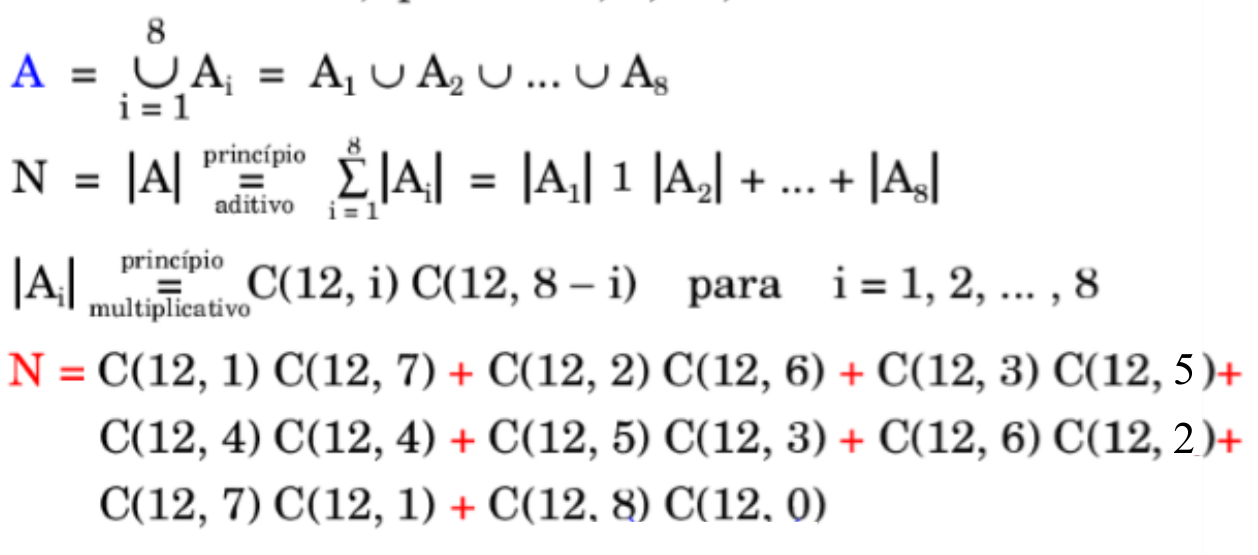
\includegraphics[width=.85\linewidth]{figs/Comb_exemplo06.png}
    \end{center}

\end{frame}



%39
\begin{frame}{Número de Combinações Simples}
    \textbf{Exemplo 7:}
    \begin{itemize}
        \item[] De quantos modos é possível dividir 20 pessoas em um grupo de 12 e um grupo de 8?
    \end{itemize}

    \pause
    \vspace{2mm}

    \textbf{Resolução:}
    \begin{itemize}
        \item[] Raciocínio 1:
        \begin{itemize}
            \item N: modos de dividir 20 em 1 grupo de 12 e outro de 8 \pause
            \item M: quantidade de grupos de 12 dentre 20 = C(20,12) \pause
            \item \underline{Dado} 1 grupo de \underline{12}, o grupo de \underline{8 fica definido}.
        \end{itemize}
    \end{itemize}

    \pause
    \vspace{2mm}
    \textbf{Resposta:}

    \begin{itemize}
        \item $N = C(20,12) = \frac{20!}{12! 8!}$
    \end{itemize}

\end{frame}


%42
\begin{frame}{Número de Combinações Simples}
    \textbf{Exemplo 7 (raciocínio 2):}
    \begin{itemize}
        \item N: modos de dividir 20 em 1 grupo de 12 e outro de 8
        \item M: quantidade de grupos de 8 dentre 20 = $C(20,8)$ \pause
        \item \underline{Dado} 1 grupo de \underline{8}, o grupo de \underline{12 fica definido}.
    \end{itemize}

    \pause
    \vspace{2mm}

    \textbf{Resposta:}

    \begin{itemize}
        \item $N = C(20,8) = \frac{20!}{8! 12!} = C(20,12)$
    \end{itemize}

\end{frame}


%43
\begin{frame}{Número de Combinações Simples}
    \textbf{Exemplo 8:}
    \begin{itemize}
        \item De quantos modos é possível dividir 20 pessoas em 2 grupos de 10?
    \end{itemize}

    \pause
    \vspace{2mm}

    \textbf{Resolução:}

    \begin{itemize}
        \item N: modos de dividir 20 em 2 grupos de 10 \pause
        \item M: quantidade de grupos de 10 dentre 20 = $C(20,10)$ \pause
        \item \underline{Dado} 1 grupo de \underline{10}, o \underline{outro grupo fica definido}.
    \end{itemize}

\end{frame}

%44
\begin{frame}{Número de Combinações Simples}
    \textbf{Exemplo 8 (continuação):}
    \begin{itemize}
        \item Diferença com o exemplo 7:
        \begin{itemize}
            \item Os 2 grupos são de 10 pessoas (estamos dividindo as 20 pessoas por 2)
        \end{itemize}
    \end{itemize}

    \pause
    \vspace{2mm}

    \textbf{Ilustração:}

    \begin{center}
        $p_1, p_2, \ldots, p_{20}$ as pessoas
    \end{center}

    \begin{itemize}
        \item a escolha $p_1, p_2, \ldots, p_{10}$ define o outro grupo $p_{11}, p_{12}, \ldots, p_{20}$
        \item a escolha $p_{11}, p_{12}, \ldots, p_{20}$ define o outro grupo  $p_1, p_2, \ldots, p_{10}$ 
    \end{itemize}

    \pause
    \vspace{2mm}

    \textbf{Resposta:}
    $$ N = \frac{C(20,10)}{2} = \frac{1}{2} \cdot \frac{20!}{10! 10!}$$
\end{frame}

%45
\begin{frame}{Número de Combinações Simples}
    \textbf{Exemplo 9:}
    \begin{itemize}
        \item Um concurso para professor tem 20 inscritos. Devem ser selecionadas 10 pessoas para realizar a prova em 1 dia e 10 para fazê-la no dia seguinte. De quantos modos é possível fazer a seleção?
    \end{itemize}

    \pause
    \vspace{2mm}

    \textbf{Resolução:}

    \begin{itemize}
        \item Relações com o exercício 8:
        \begin{itemize}
            \item Semelhança: Escolha de 2 grupos de 10 entre 20
            \item Diferença: Existe uma ordem entre os grupos determinada pelo dia da prova.
        \end{itemize}
    \end{itemize}

\end{frame}

%46
\begin{frame}{Número de Combinações Simples}
    \textbf{Exemplo 9 (continuação):}
    \begin{itemize}
        \item a escolha $p_1, p_2, \ldots, p_{10}$ (1º dia) define o grupo $p_{11}, p_{12}, \ldots, p_{20}$ (2º dia)
        \item a escolha $p_{11}, p_{12}, \ldots, p_{20}$ (1º dia) define o grupo $p_1, p_2, \ldots, p_{10}$ (2º dia)
    \end{itemize}

    \pause
    \vspace{2mm}

    \textbf{Resolução:}

    \begin{itemize}
        \item Relações com o exercício 8:
        \begin{itemize}
            \item Semelhança: Escolha de 2 grupos de 10 entre 20
            \item Diferença: Existe uma ordem entre os grupos determinada pelo dia da prova.
        \end{itemize}
    \end{itemize}

    \pause

    \vspace{2mm}

    \textbf{Resposta:}

    \begin{itemize}
        \item Tem-se $C(20,10)$ possibilidades de seleção.
    \end{itemize}
\end{frame}

\end{document}